\chapter{Basics}\label{ch:K01_Basics}


\begin{myexercise}\label{myexercise:kaufpreis_haus}
Sie wollen ein Haus in der Schweiz kaufen. Der Kaufpreis beträgt $k$ Franken. Sie kaufen das Haus mit $E$ Franken Ihres gesparten Geldes (Eigenkapital) und der Restbetrag wird durch die Aufnahme einer Hypothek von $h := k - E$ Franken gedeckt. 

Die Tragbarkeitsrechnung in der Schweiz prüft, ob die Kosten einer Immobilie langfristig finaziell tragbar (bezahlbar) sind. Banken und andere Kreditinstitute verwenden diese (sehr grobe) Berechnung, um sicherzustellen, dass Sie Ihre Hypothek auch dann noch bezahlen könnten, falls die Zinsen steigen würden. Als Faustregel gilt, dass die jährlichen (kalkulatorischen\footnote{Der Begriff \textit{Kalkulatorisch} bedeutet in diesem Zusammenhang, dass dieser Betrag nach bestimmten Vorgaben berechnet wird und überhaupt nicht den tatsächlichen Kosten entsprechen muss.}) Wohnkosten nicht mehr als $1 / 3$ Ihres \textcolor{ForestGreen}{Bruttojahreseinkommens} ($b$) ausmachen dürfen.

Die kalkulatorischen jährlichen Wohnkosten setzten sich als die Summe der folgenden drei Positionen zusammen:
\begin{itemize}
	\item \textcolor{NavyBlue}{Kalkulatorischer Zins}: $5$ Prozent des Hypothekenbetrags $h$, also $5$ Prozent von $k - E$
	\item \textcolor{Magenta}{Nebenkosten}: $1$ Prozent des Kaufpreises $k$
	\item \textcolor{Red}{Amortisation}: Falls die aufgenommene Hypothek grösser als $2/3$ des Kaufpreises $k$ ist, muss der darüberliegende Betrag $h - (2 / 3) k$ nach $15$ Jahren zurückbezahlt sein. Die Bank rechnet also hierführ mit jährlichen Kosten $a$ für die Amortisation von
	\begin{align*}
		a := \frac{h - (2 / 3) k}{15} = \frac{(k - E) - (2 / 3) k}{15} 
	\end{align*}
	und mit $a := 0$, falls die Hypothek $2 / 3$ des Kaufpreises nicht übersteigt.
\end{itemize}
Zusammengefasst muss also die Ungleichung
\begin{align*}
	\frac{\text{\textcolor{ForestGreen}{Brutto-Jahreseinkommen}}}{3} \geq \text{\textcolor{NavyBlue}{Kalkulatorischer Zins}} + \text{\textcolor{Magenta}{Nebenkosten}} + \text{\textcolor{Red}{Amortisation}}
\end{align*}
oder anderst geschrieben
\begin{align*}
	b / 3 \geq 0.05(k - E) + 0.01k + \max\lrc{0, (k/3 - E) / 15}
\end{align*}
erfüllt sein. Wir wollen unsere Berechnung möglichst allgemein halten und ersetzen die kalkulatorische Hypothekenrate von $0.05$ durch die positive Variable $\alpha$ und die kalkulatorische Nebenkostenrate $0.01$ durch die positive Variable $\beta$:
\begin{align}\label{eq:Ungleichung_k}
	b / 3 \geq \alpha (k - E) + \beta k + \max\lrc{0, (k/3 - E) / 15}.
\end{align}

Nun gibt es für den Kaufpreis $k$ noch eine weitere Zusatzbedingung: \textbf{Der Kaufpreis darf nicht höher sein als das Fünffache des Eigenkapitals}.

\begin{enumerate}
	\item Lösen Sie die Ungleichung nach $k$ auf. Natürlich wird $k$ abhängig sein von $E, b, \alpha$ und $\beta$.
	\item Schreiben Sie eine Funktion \lstinline|max_kaufpreis(E, b, alpha, beta)|, welche für gegebene Werte von $E, b, \alpha$ und $\beta$ den maximal tragbaren Kaufpreis berechnet und mit \lstinline|return| zurück gibt.
	\item Geben Sie eine Formel für das maximal tragbare $k$ in Excel an, falls $E$ in \texttt{A1}, $b$ in \texttt{A2}, $\alpha$ in \texttt{A3} und $\beta$ in \texttt{A4} gespeichert sind.
\end{enumerate}

\begin{myanswer}
	Diese Musterlösung finden Sie in \cref{sec:K01_sol}.
\end{myanswer}
\end{myexercise}


\begin{mychallenge}\label{mychallenge:Eigenleistung}
Angenommen Sie kaufen ein Haus mit nennenswertem Renovationsbedarf. Falls Sie planen diese Arbeiten in Eigenleistung durchzuführen, rechnen Ihnen Banken für diese Eigenleistung \enquote{bis zu 5 Prozent des Kaufpreises als Eigenkapitel an}. Genauer (aber weniger intuitiv) gesagt, müssen Sie in der Tragbarkeitsrechnung (kalkulatorisch) nur noch mit einem Hypothekenbetrag von $k - (\gamma k + E)$ rechnen anstelle von $k - E$, wobei $\gamma\in\lrs{0,0.05}$. Falls $\gamma\neq 0$ kann dadurch natürlich ein grösserer maximaler Kaufpreis finanziert werden. Passen Sie Ungleichung \ref{eq:Ungleichung_k} an, sodass sie diesen Term $\gamma$ korrekt berücksichtig. Lösen Sie die neue Ungleichung nach $k_{\text{max}}$ auf.
\begin{myanswer}
    Die angepasste Ungleichung ist:
    \begin{align*}
         b / 3 \geq \alpha ( k - (\gamma k + E)) + \beta k + \max\lrc{0, ( k/3 - (\gamma k + E)) / 15}.
    \end{align*}
    Aufgelöst nach $k$ (unter Berücksichtigung aller anderen Bedingungen):
        		{\scriptsize
		\begin{align*}
			k_{\text{max}} = \max\lrc{\min\lrc{\min\lrc{\frac{b/3 + \alpha E}{\alpha (1 - \gamma) + \beta}, \frac{15b + 45\alpha E + 3E}{45\alpha (1 - \gamma) + 45\beta + 1 - 3\gamma}}, 5E}, E}
		\end{align*}
                }
\end{myanswer}
\end{mychallenge}

\iftoggle{exerciseonly}{}{%
	\clearpage

	\section{Längere Lösungen}\label{sec:K01_sol}

		\begin{myanswer}[myexercise:kaufpreis_haus]
			\begin{enumerate}
				\item 

		Wir ignorieren zunächst die Bedingung $k \leq 5E$ und betrachten die Ungleichung \ref{eq:Ungleichung_k}. Dabei unterscheiden wir zwei Fälle:

		\begin{description}
			\item[Fall 0: $\max\lrc{0, -E + k/3} = 0$, also $k \leq 3E$ (keine Amortisationspflicht):] Die Ungleichung \ref{eq:Ungleichung_k} vereinfacht sich in diesem Fall zu
\begin{align*}
\frac{b}{3} &\geq \alpha(k - E) + \beta k \\
\frac{b}{3} &\geq \alpha k - \alpha E + \beta k \\
\frac{b}{3} + \alpha E &\geq k(\alpha + \beta) \\
k &\leq \frac{b/3 + \alpha E}{\alpha + \beta} := \textcolor{Salmon}{k_0}
\end{align*}
\item[Fall 1:$\max\lrc{0, -E + k/3} = -E + k/3$, also $k > 3E$ (Amortisationspflicht):] In diesem Fall ist $\max\lrc{0, -E + k/3} = -E + k/3$. Die Ungleichung vereinfacht sich in diesem Fall zu
\begin{align*}
\frac{b}{3} &\geq \alpha\lr{k - E} + \beta k + \frac{k/3 - E}{15} \\
\frac{b}{3} &\geq \alpha k - \alpha E + \beta k + \frac{k}{45} - \frac{E}{15} \\
\frac{b}{3} + \alpha E + \frac{E}{15} &\geq k\lr{\alpha + \beta + \frac{1}{45}} \\
\frac{15b + 45\alpha E + 3E}{45} &\geq k\lr{\frac{45\alpha + 45\beta + 1}{45}} \\
15b + 45\alpha E + 3E &\geq k\lr{45\alpha + 45\beta + 1} \\
k &\leq \frac{15b + 45\alpha E + 3E}{45\alpha + 45\beta + 1} := \textcolor{Goldenrod}{k_1}
\end{align*}
\end{description}
Damit $k$ die ursprüngliche Ungleichung \ref{eq:Ungleichung_k} erfüllt, muss $k$ kleiner oder gleich dem kleineren der beiden Beträge $\textcolor{Salmon}{k_0}$ und $\textcolor{Goldenrod}{\textcolor{Goldenrod}{k_1}}$ sein. Also finden wir unter der Berücksichtigung der bislang ignorierten Bedingung $k \leq 5E$:
	\begin{align*}
		k := \min\lrc{\min\lrc{\textcolor{Salmon}{k_0}, \textcolor{Goldenrod}{k_1}}, 5E}.
	\end{align*}

Beachten Sie, dass Fall 0 die Beziehung $k < E$ nicht ausschliesst. In diesem Fall wäre aber $k - E < 0$ und die Hypothek wäre somit negativ. Eine negative Hypothek wäre dann eher als Guthaben zu verstehen und natürlich macht die Tragbarkeitssberechnung für ein Guthaben keinen Sinn. In diesem Fall ist der maximale Kaufpreis $E$ (wir bezhalen einfach alles mit Eigenkapital und nehmen gar keine Hypothek auf). Die Gleichung $\frac{b/3 + \alpha E}{\alpha + \beta} \stackrel{!}{=} E$ (aufgelöst nach $b$) zeigt, dass sich der maximal tragbare Kaufpreis mit steigendem Lohn $b$ nicht erhöht, solange noch $b \leq 3\alpha$ ist.

	Um den Spezialfall $k - E < 0$ (negative Hypothek) auszuschliessen, müssen wir noch das Maximum zwischen $k$ und $E$ nehmen, also
	\begin{mysummary}
		{\scriptsize
		\begin{align*}
			k_{\text{max}} = \max\lrc{\min\lrc{\min\lrc{\textcolor{Salmon}{k_0}, \textcolor{Goldenrod}{k_1}}, 5E}, E} = \max\lrc{\min\lrc{\min\lrc{\frac{b/3 + \alpha E}{\alpha + \beta}, \frac{15b + 45\alpha E + 3E}{45\alpha + 45\beta + 1}}, 5E}, E}
		\end{align*}
		}
	\end{mysummary}

	\item 
	Die entsprechende Python-Funktion ist gegeben durch:
	\lstinputlisting{Grundlagen_Info/00_Programmieren/Skript/Code/K04_Functions/max_kaufpreis.py}
	
		\begin{figure}[H]
		\centering
		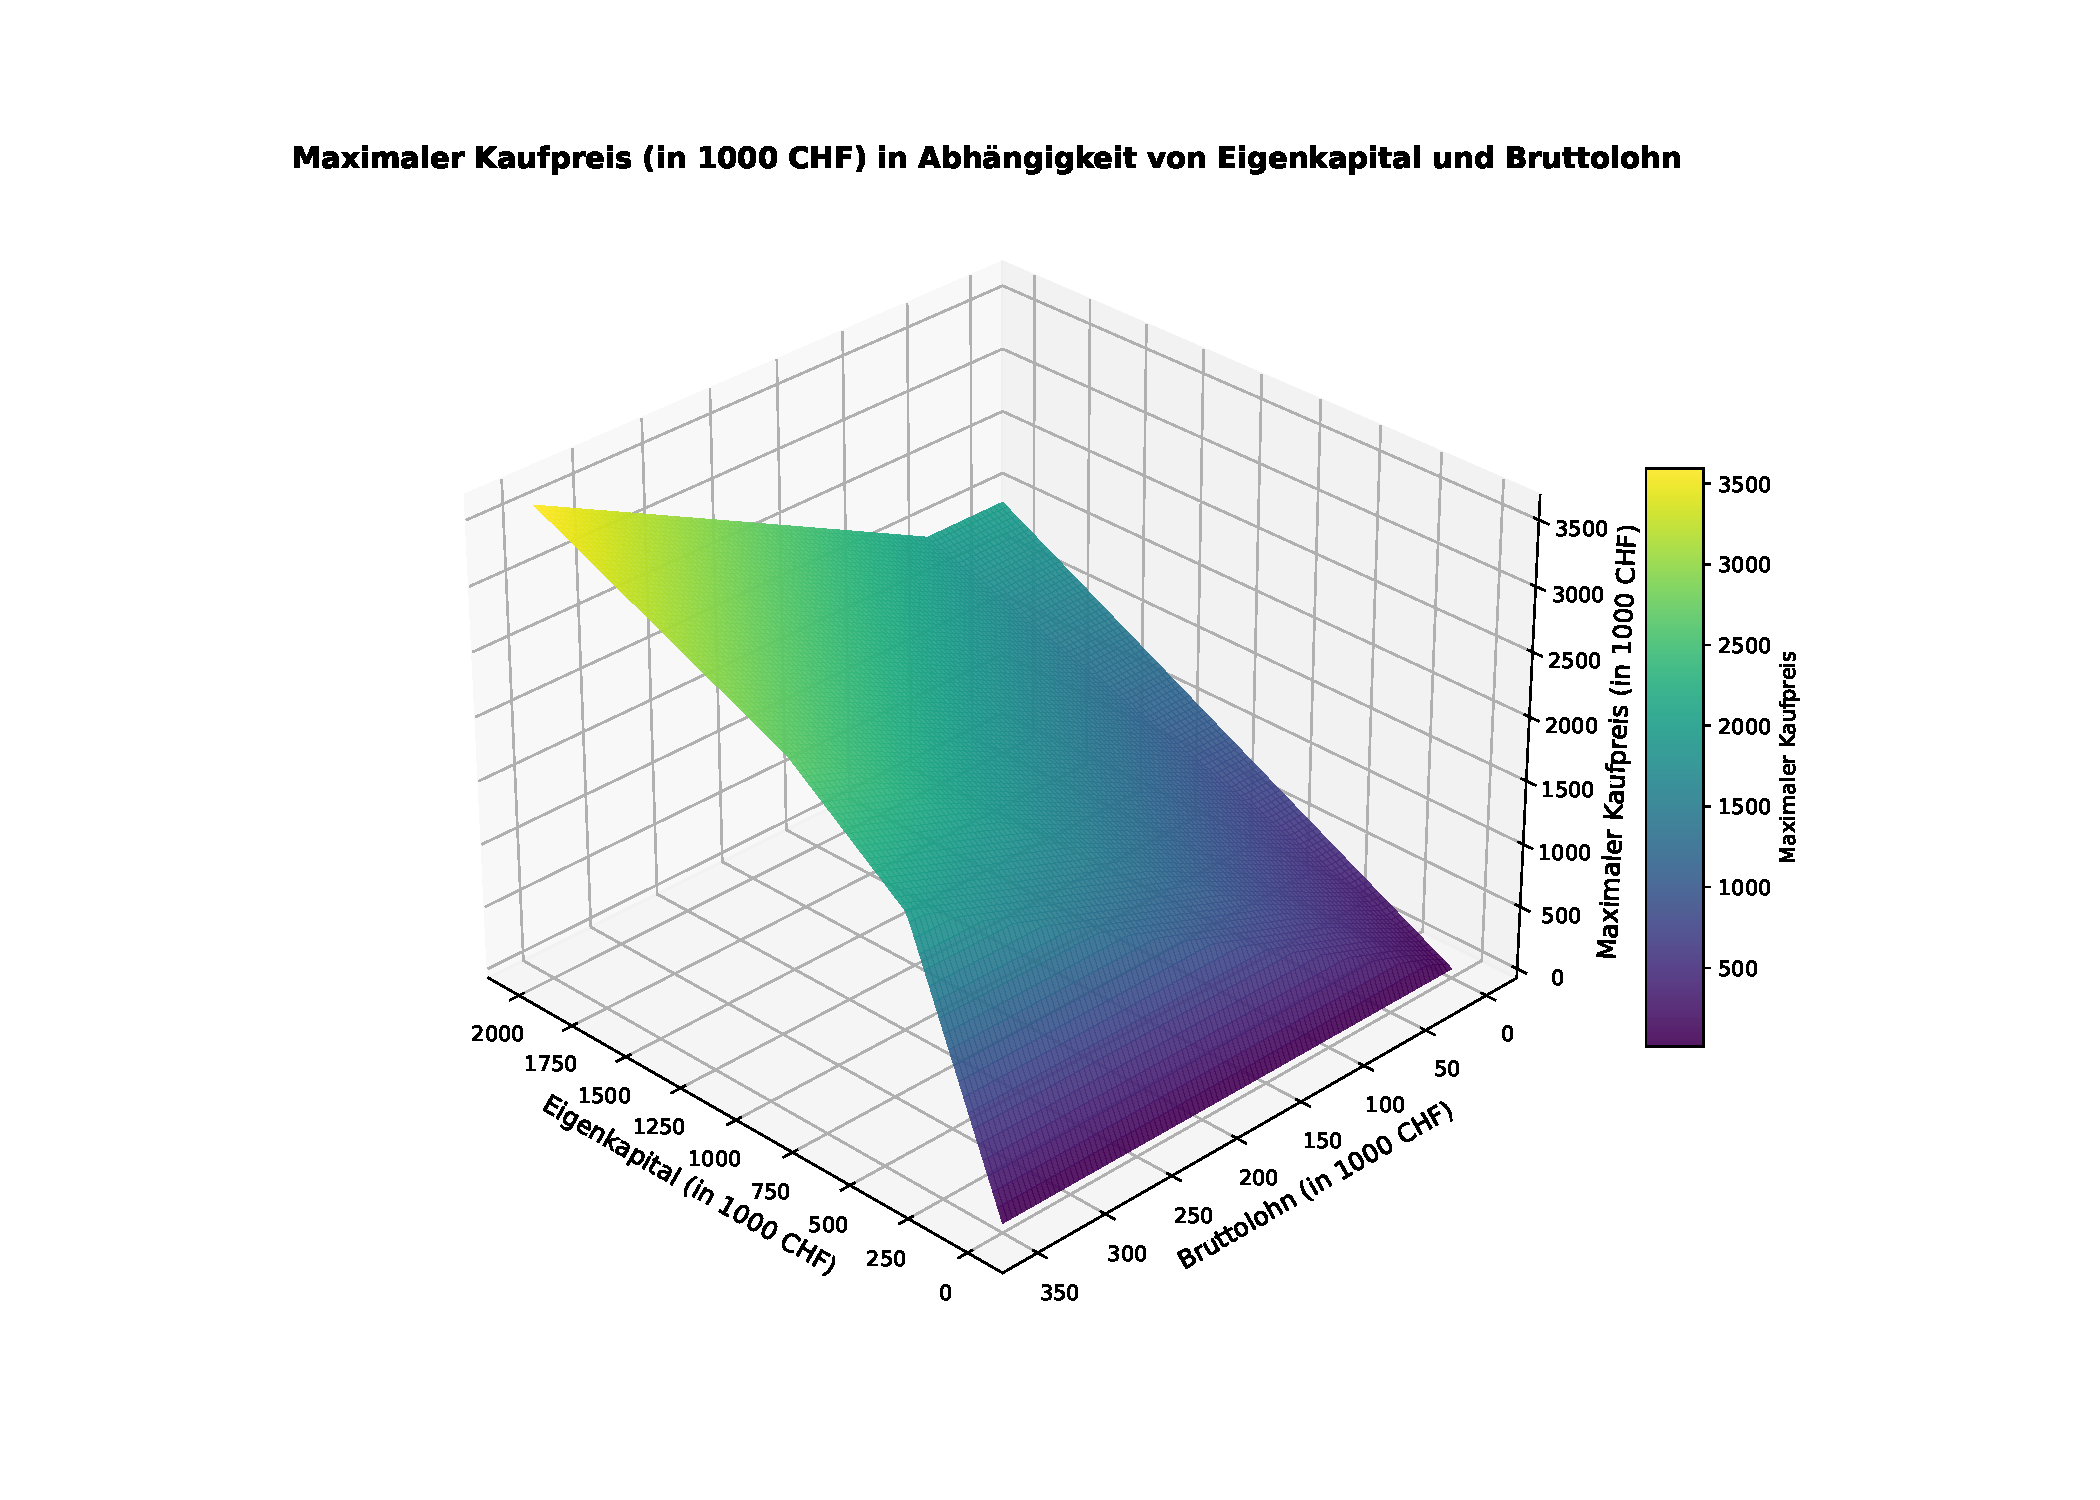
\includegraphics[width=0.9\textwidth]{Grundlagen_Info/00_Programmieren/Skript/Code/K04_Functions/max_kaufpreis_3d_plot.pdf}
		\caption{3D-Plot des maximalen Kaufpreises abhängig vom Jahresbruttolohn und dem Eigenkapital für $\alpha = 0.05, \beta = 0.01$.}
	\end{figure}
	
	\item Und schliesslich die Formel in Excel:
	
	\lstinline[basicstyle=\ttfamily\scriptsize]{MAX(MIN(MIN((A2/3 + A3 * A1) / (A3 + A4), (15 * A2 + 45 * A3 * A1 + 3 * A1) / (45 * A3 + 45 * A4 + 1)), 5 * A1), A1)}
	\end{enumerate}
	\end{myanswer}

} %